\documentclass[border=10pt]{standalone}

\usepackage{tikz}
\usepackage{tikzsymbols}
\usetikzlibrary{calc,patterns,shapes.geometric}

\def\centerarc[#1](#2)(#3:#4:#5){\draw[#1] ($(#2)+({#5*cos(#3)},{#5*sin(#3)})$) arc (#3:#4:#5);}

\begin{document}
	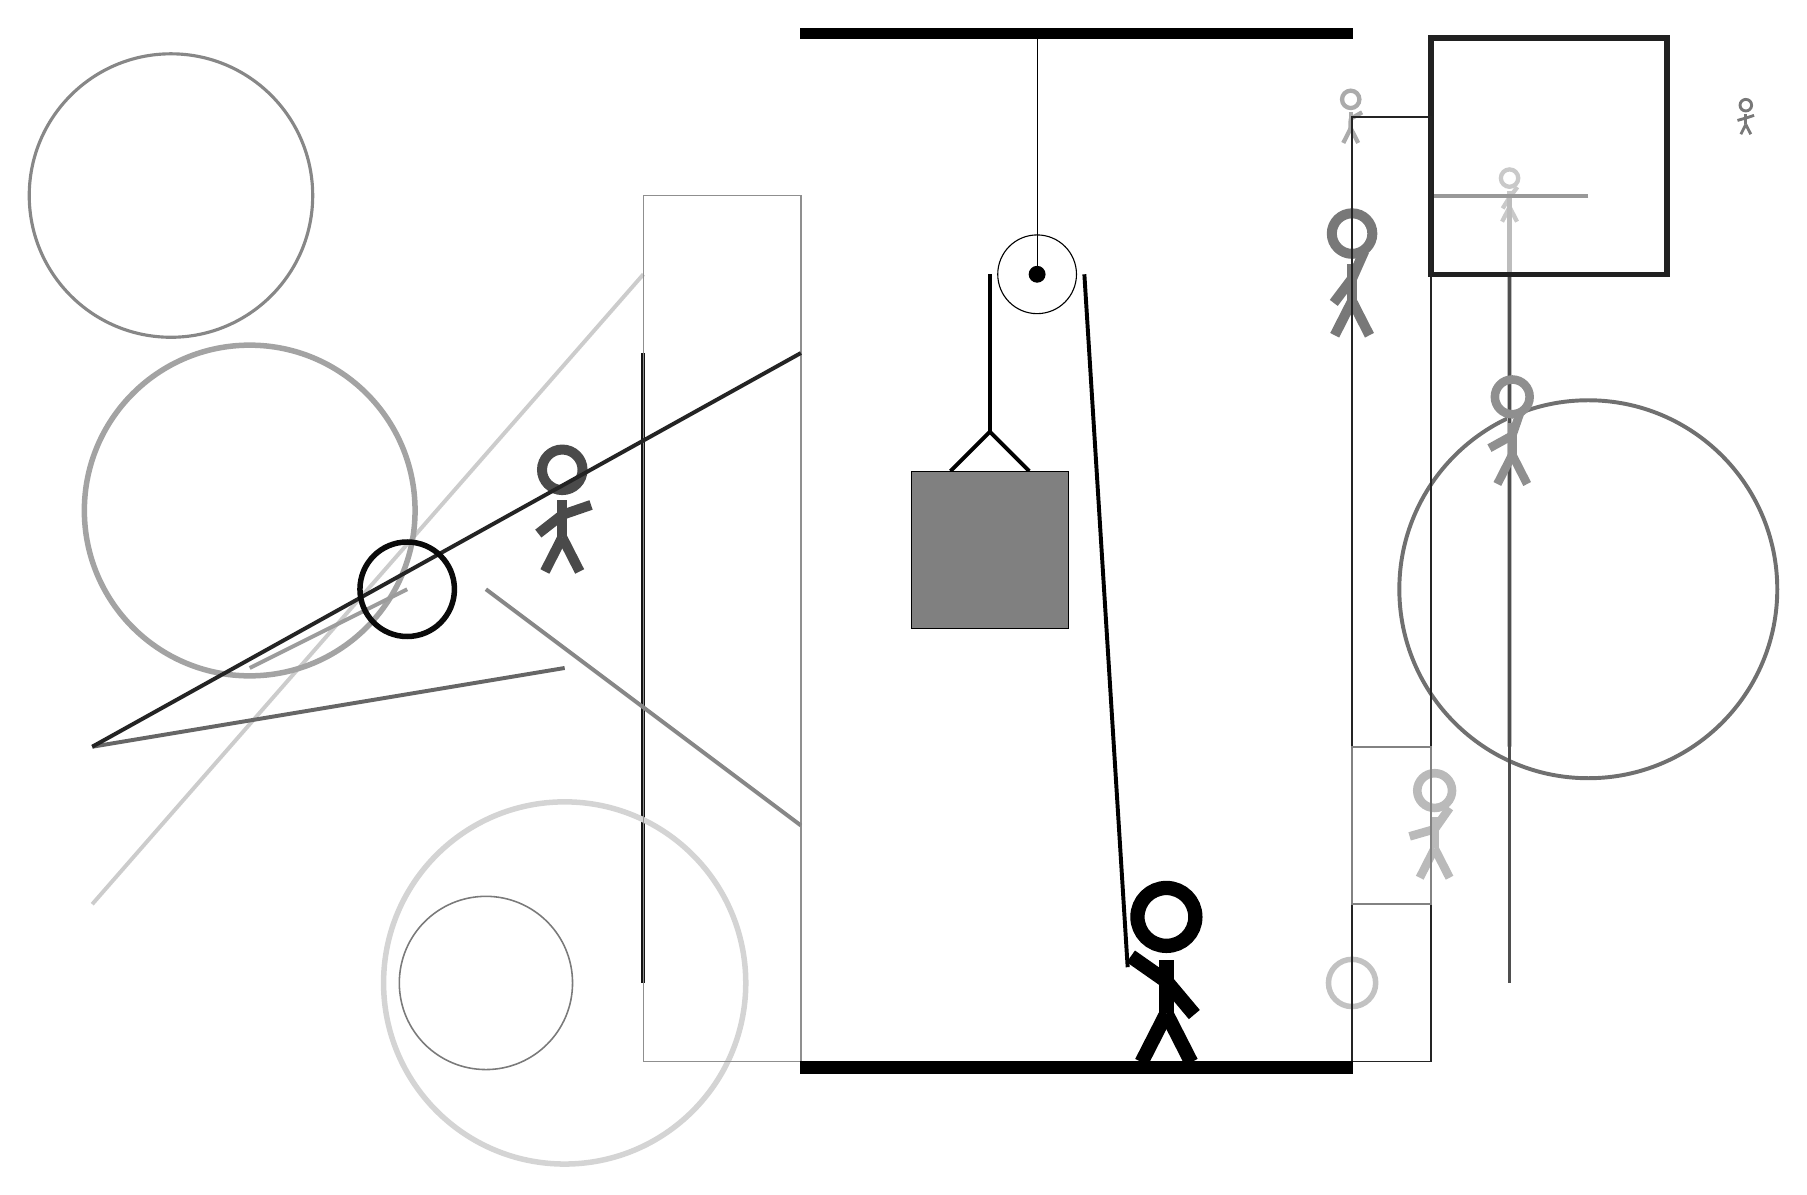
\begin{tikzpicture}
		%%%%% START %%%%%
		
		\draw[fill=black] (-2, 10) rectangle (5, 10.125);
		
		\draw [line width=0.5mm, color=black!56](8, 3) circle (2.4);
		
		\node[line width=0.5mm, color=black!21] at (7, 8) {\Strichmaxerl[3][58][53]};
		\draw[line width=0.5mm, color=black!20](-4, 7) -- (-11, -1);
		\draw[line width=0.5mm, color=black!60](-5, 2) -- (-11, 1);
		\draw [line width=0.7mm, color=black!24](5, -2) circle (0.3);
		\draw[line width=0.5mm, color=black!92](-4, 6) -- (-4, -2);
		\draw [line width=0.2mm, color=black!52](-6, -2) circle (1.1);
		\node[line width=0.4mm, color=black!71] at (-5, 4) {\Strichmaxerl[7][38][19]};
		\draw[line width=0.6mm, color=black!26] (7, 8) rectangle (7, 1);
		
		\node[line width=0.6mm, color=black!53] at (5, 7) {\Strichmaxerl[7][53][66]};
		\draw [line width=0.7mm, color=black!17](-5, -2) circle (2.3);
		\draw [line width=0.7mm, color=black!36](-9, 4) circle (2.1);
		\draw[line width=0.2mm, color=black!44] (-2, 8) rectangle (-4, -3);
		
		\draw[line width=0.5mm, color=black!39](-7, 3) -- (-9, 2);
		\draw[line width=0.5mm, color=black!86](-2, 6) -- (-11, 1);
		\draw[line width=0.5mm, color=black!40](8, 8) -- (6, 8);
		
		\draw[line width=0.3mm, color=black!69] (7, 7) rectangle (7, -2);
		\node[line width=0.3mm, color=black!27] at (6, 0) {\Strichmaxerl[6][16][55]};
		\node[line width=0.2mm, color=black!53] at (10, 9) {\Strichmaxerl[2][16][18]};
		\draw [line width=0.4mm, color=black!47](-10, 8) circle (1.8);
		\draw[line width=0.7mm, color=black!87] (6, 7) rectangle (9, 10);
		\node[line width=0.5mm, color=black!44] at (7, 5) {\Strichmaxerl[6][29][71]};
		
		\node[line width=0.4mm, color=black!33] at (5, 9) {\Strichmaxerl[3][88][29]};
		\draw[line width=0.2mm, color=black!86] (6, -3) rectangle (5, 9);
		\draw[line width=0.5mm, color=black!47](-6, 3) -- (-2, 0);
		\draw [line width=0.7mm, color=black!96](-7, 3) circle (0.6);
		\draw[line width=0.3mm, color=black!49] (6, 1) rectangle (5, -1);
		
		\draw (1, 7) circle (0.5);
		\draw[fill=black] (1, 7) circle (0.1);
		\draw (1, 10) -- (1, 7);
		
		\draw[line width=0.5mm] (-0.1, 4.5) -- (0.4, 5.0) -- (0.9, 4.5);
		\draw[fill=black!50] (-0.6, 4.5) rectangle (1.4, 2.5);
		
		\draw[line width=0.5mm] (0.4, 7) -- (0.4, 5.0);
		\centerarc[line width=0.5mm](1, 7)(0:180:0.6);
		\draw[line width=0.5mm](1.6, 7) -- (2.15, -1.8);
		
		\node at (2.6, -1.9) {\Strichmaxerl[10][-35][-50]};
		
		\draw[fill=black] (-2, -3) rectangle (5, -3.15);
		
		%%%%% END %%%%%
	\end{tikzpicture}
\end{document}